\documentclass[12pt]{article} 
\usepackage[margin=1in]{geometry} 
\usepackage{graphicx} 
\usepackage{hyperref} 
\usepackage{tocloft}
\usepackage{enumitem}
\usepackage{mathptmx} % Times New Roman
\usepackage{setspace}
\usepackage{fancyhdr} % Header and footer
\usepackage[indonesian]{babel}
\usepackage{caption}
\captionsetup[table]{name=Tabel}
\captionsetup[figure]{name=Gambar}

\renewcommand{\contentsname}{Daftar Isi}

\title{Laporan Evaluasi Tengah Semester\\Pemrograman Jaringan C} 
\author{Muhammad Daffa' Ashdaqfillah (5025211015)} 
\date{\today} 

\pagestyle{fancy}
\fancyhf{} % Clear existing header/footer
\rhead{Evaluasi Tengah Semester - Progjar C}
\rfoot{\thepage}
\lfoot{Muhammad Daffa Ashdaqfillah - 5025211015}
\renewcommand{\footrulewidth}{0.4pt}

\begin{document}

% Halaman Cover
\begin{titlepage}
    \centering
    {\scshape\Large Laporan Pengerjaan\par}
    \vspace{0.4cm}
    {\huge\bfseries Evaluasi Tengah Semester\par}
    \vspace{0.1cm}
    {\large\bfseries Pemrograman Jaringan C\par}
    \vspace{1cm}
    \vspace{1.5cm}
    
\includegraphics[width=0.6\textwidth]{img/logo_its.png}\par\vspace{1cm}
    \vspace{1cm}
    \vspace{1.5cm}
    {\large\bfseries Muhammad Daffa' Ashdaqfillah (5025211015)\par}
    {\scshape\LARGE Institut Teknologi Sepuluh Nopember \par}
    \vfill
    {\large Surabaya\par}
    {\large 28 Mei 2024\par}
    \end{titlepage}
\newpage

\setcounter{page}{2} % Mulai penomoran halaman setelah sampul

% Daftar Isi
\tableofcontents
\newpage

\section{Pendahuluan}

Laporan ini mengevaluasi kinerja berbagai implementasi server web, yaitu menggunakan \textit{multithreading}, \textit{multiprocessing}, dan varian \textit{secure} dari keduanya. Kode server yang dievaluasi (disajikan sebelumnya) merupakan modifikasi dari contoh yang disediakan dalam \textit{progjar5}. Server ini dirancang untuk menangani permintaan HTTP sederhana, menjadikannya dasar yang ideal untuk memahami bagaimana model konkurensi (\textit{multithreading} dan \textit{multiprocessing}) memengaruhi kinerja server dalam skenario beban kerja yang berbeda.

\subsection{Tujuan}

Tujuan utama dari evaluasi ini adalah:

\begin{enumerate}
    \item \textbf{Membandingkan Kinerja:} Menganalisis secara kuantitatif perbedaan kinerja antara model \textit{multithreading} dan \textit{multiprocessing}, baik dalam versi standar maupun yang telah diamankan (\textit{secure}).
    \item \textbf{Mengukur Skalabilitas:} Menilai bagaimana setiap implementasi server menangani peningkatan jumlah permintaan bersamaan (\textit{concurrency}).
    \item \textbf{Memahami Faktor-Faktor Kinerja:} Mengidentifikasi metrik kinerja utama yang dipengaruhi oleh pilihan model konkurensi dan keamanan, termasuk waktu respons, \textit{throughput}, dan penggunaan sumber daya.
    \item \textbf{Memberikan Rekomendasi:} Berdasarkan hasil evaluasi, memberikan rekomendasi tentang model konkurensi yang paling sesuai untuk berbagai skenario penggunaan server web.
\end{enumerate}

Evaluasi ini menggunakan Siege untuk menghasilkan beban kerja yang realistis dan mengumpulkan metrik kinerja yang relevan.

\subsection{Repositori Kode}

Kode sumber yang digunakan dalam evaluasi ini, dapat ditemukan di repositori GitHub berikut:
\href{https://github.com/daf2a/Laporan_ETS_Progjar}{Laporan\_ETS\_Progjar}

\newpage

\section{Metodologi}
\subsection{Pengaturan Eksperimen}
Uji coba dilakukan pada mesin virtual dengan spesifikasi berikut:

\begin{table}[h]
\centering
\caption{Spesifikasi Mesin Virtual}
\label{tab:vm_specs}
\begin{tabular}{|l|l|}
\hline
\textbf{Komponen} & \textbf{Spesifikasi} \\ \hline
Sistem Operasi & Linux (5.15.146.1-microsoft-standard-WSL2) \\ 
Prosesor & AMD Ryzen 7 4800H with Radeon Graphics (16 cores, 32 threads) \\
RAM & 5.5 GiB \\
Penyimpanan & 1007 GB (overlay), 340 GB (E:) \\
\hline
\end{tabular}
\end{table}

Server web dijalankan pada mesin virtual ini. Pengujian kinerja dilakukan dari mesin lain yang terhubung ke jaringan lokal yang sama. 

\begin{figure}[h!]
\centering
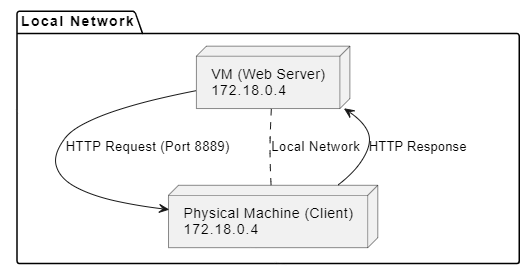
\includegraphics[width=0.8\textwidth]{img/architecture_diagram.png}
\caption{Diagram Arsitektur Eksperimen}
\label{fig:arch}
\end{figure}

Gambar \ref{fig:arch} mengilustrasikan arsitektur percobaan. Mesin penguji (client) dan mesin yang menjalankan server web (virtual machine) terhubung ke jaringan lokal yang sama. Pengujian kinerja dilakukan dengan mengirimkan permintaan HTTP ke server web menggunakan Siege.

\subsection{Pengukuran Kinerja}

Pengukuran kinerja dilakukan menggunakan \texttt{Siege}, alat pengujian HTTP yang digunakan untuk mensimulasikan banyak pengguna yang mengakses server secara bersamaan.

\subsubsection{Parameter Pengujian}

Pengujian dilakukan dengan durasi 30 detik (`-t 30S`) pada setiap iterasi. Tingkat konkurensi (jumlah pengguna virtual yang mengakses server secara bersamaan) divariasikan untuk melihat bagaimana kinerja server berubah seiring dengan meningkatnya beban. Tingkat konkurensi yang digunakan adalah 10, 50, 100, 150, dan 200 (`-c 10`, `-c 50`, dst.).

\subsubsection{Perintah yang Digunakan}

Perintah dasar yang digunakan untuk menjalankan pengujian HTTP adalah sebagai berikut:

\texttt{siege -c [TINGKAT\_KONKURENSI] -t 30S http://[ALAMAT\_IP\_SERVER]:8889/}
\\ \\
Sedangkan perintah untuk HTTPS sebagai berikut:

\texttt{siege -c [TINGKAT\_KONKURENSI] -t 30S https://[ALAMAT\_IP\_SERVER]:8443/}

\subsection{Modifikasi Kode Sumber}

Pada semua kode, dhilangkan beberapa overhead seperti print/mencetak log seluruh isi direktori/folder untuk mempercepat proses.



\newpage
\section{Hasil dan Analisis}
\subsection{Perbandingan Kinerja}
% Sajikan data kinerja Anda dalam format tabel, seperti yang diminta.
Berikut adalah hasil pengujian kinerja untuk server web dengan model konkurensi \textit{multithreading} dan \textit{multiprocessing} dalam versi standar dan \textit{secure}.

\begin{table}[h!]
    \captionsetup{justification=raggedright,singlelinecheck=false}
    \caption{Kinerja Server Web (\textbf{Thread non Secure})}
    \label{tab:thread_secure_performance_1}
    \begin{tabular}{c|ccccc}
    \hline
    \textbf{Concurrency} & \textbf{Failed} & \textbf{Total} & \textbf{Requests} & \textbf{Time/Request} & \textbf{Transfer} \\
    \textbf{Level} & \textbf{Requests} & \textbf{Transactions} & \textbf{/s} & \textbf{(ms)} & \textbf{Rate (Mb/s)} \\
    \hline
    10 & 0 & 155 & 5.19 & 1840 & 0.00 \\
    50 & 0 & 144 & 4.96 & 3990 & 0.00 \\
    100 & 1 & 122 & 4.13 & 5040 & 0.00 \\
    150 & 2 & 106 & 3.64 & 5540 & 0.00 \\
    200 & 0 & 111 & 3.75 & 5800 & 0.00 \\
    \hline
    \end{tabular}
    \end{table}

    \begin{table}[h!]
    \label{tab:thread_secure_performance_2}
    \begin{tabular}{c|cccc}
    \hline
    \textbf{Concurrency} & \textbf{Longest} & \textbf{Shortest} & \textbf{Throughput} & \textbf{Total} \\
    \textbf{Level} & \textbf{Transactions (ms)} & \textbf{Transactions (ms)} & \textbf{} & \textbf{Time (ms)} \\
    \hline
    10 & 8.94 & 0.49 & 0.00 & 29840 \\
    50 & 24.85 & 0.45 & 0.00 & 29020 \\
    100 & 18.85 & 0.00 & 0.00 & 29510 \\
    150 & 19.86 & 0.00 & 0.00 & 29120 \\
    200 & 19.43 & 0.00 & 0.00 & 29610 \\
    \hline
    \end{tabular}
    \end{table}

\begin{table}[h!]
    \captionsetup{justification=raggedright,singlelinecheck=false}
    \caption{Kinerja Server Web (\textbf{Thread Secure})}
    \label{tab:thread_secure_performance_1}
    \begin{tabular}{c|ccccc}
    \hline
    \textbf{Concurrency} & \textbf{Failed} & \textbf{Total} & \textbf{Requests} & \textbf{Time/Request} & \textbf{Transfer} \\
    \textbf{Level} & \textbf{Requests} & \textbf{Transactions} & \textbf{/s} & \textbf{(ms)} & \textbf{Rate (Mb/s)} \\
    \hline
    10 & 0 & 345 & 11.60 & 750 & 0.34 \\
    50 & 0 & 138 & 4.66 & 3870 & 0.00 \\
    100 & 0 & 83 & 2.83 & 7960 & 0.00 \\
    150 & 0 & 43 & 1.44 & 4840 & 0.00 \\
    200 & 0 & 65 & 2.19 & 5190 & 0.00 \\
    \hline
    \end{tabular}
    \end{table}
    
    \begin{table}[h!]
    \label{tab:thread_secure_performance_2}
    \begin{tabular}{c|cccc}
    \hline
    \textbf{Concurrency} & \textbf{Longest} & \textbf{Shortest} & \textbf{Throughput} & \textbf{Total} \\
    \textbf{Level} & \textbf{Transactions (ms)} & \textbf{Transactions (ms)} & \textbf{} & \textbf{Time (ms)} \\
    \hline
    10 & 8.47 & 0.02 & 0.00 & 29750 \\
    50 & 18.02 & 0.00 & 0.00 & 29620 \\
    100 & 25.62 & 0.00 & 0.00 & 29330 \\
    150 & 18.24 & 0.00 & 0.00 & 29790 \\
    200 & 17.88 & 0.00 & 0.00 & 29640 \\
    \hline
    \end{tabular}
    \end{table}

\begin{table}[h!]
    \captionsetup{justification=raggedright,singlelinecheck=false}
    \caption{Kinerja Server Web (\textbf{Process non Secure})}
    \label{tab:thread_secure_performance_1}
    \begin{tabular}{c|ccccc}
    \hline
    \textbf{Concurrency} & \textbf{Failed} & \textbf{Total} & \textbf{Requests} & \textbf{Time/Request} & \textbf{Transfer} \\
    \textbf{Level} & \textbf{Requests} & \textbf{Transactions} & \textbf{/s} & \textbf{(ms)} & \textbf{Rate (Mb/s)} \\
    \hline
    10 & 0 & 149 & 4.98 & 1930 & 0.00 \\
    50 & 0 & 129 & 4.38 & 9050 & 0.00 \\
    100 & 0 & 119 & 4.00 & 14140 & 0.00 \\
    150 & 0 & 34 & 1.14 & 25260 & 0.00 \\
    200 & 0 & 96 & 3.30 & 16420 & 0.00 \\
    \hline
    \end{tabular}
    \end{table}
    
\begin{table}[h!]
    \label{tab:thread_secure_performance_2}
    \begin{tabular}{c|cccc}
    \hline
    \textbf{Concurrency} & \textbf{Longest} & \textbf{Shortest} & \textbf{Throughput} & \textbf{Total} \\
    \textbf{Level} & \textbf{Transactions (ms)} & \textbf{Transactions (ms)} & \textbf{} & \textbf{Time (ms)} \\
    \hline
    10 & 4.41 & 0.41 & 0.00 & 29940 \\
    50 & 12.88 & 0.87 & 0.00 & 29430 \\
    100 & 25.08 & 1.59 & 0.00 & 29730 \\
    150 & 29.64 & 0.00 & 0.00 & 29950 \\
    200 & 28.97 & 0.00 & 0.00 & 29100 \\
    \hline
    \end{tabular}
    \end{table}

    \begin{table}[h!]
    \captionsetup{justification=raggedright,singlelinecheck=false}
    \caption{Kinerja Server Web (\textbf{Process Secure})}
    \label{tab:thread_secure_performance_1}
    \begin{tabular}{c|ccccc}
    \hline
    \textbf{Concurrency} & \textbf{Failed} & \textbf{Total} & \textbf{Requests} & \textbf{Time/Request} & \textbf{Transfer} \\
    \textbf{Level} & \textbf{Requests} & \textbf{Transactions} & \textbf{/s} & \textbf{(ms)} & \textbf{Rate (Mb/s)} \\
    \hline
    10 & 0 & 345 & 11.60 & 750 & 0.34 \\
    50 & 0 & 138 & 4.66 & 3870 & 0.00 \\
    100 & 0 & 83 & 2.83 & 7960 & 0.00 \\
    150 & 0 & 43 & 1.44 & 4840 & 0.00 \\
    200 & 0 & 65 & 2.19 & 5190 & 0.00 \\
    \hline
    \end{tabular}
    \end{table}
    
    \begin{table}[h!]
    \label{tab:thread_secure_performance_2}
    \begin{tabular}{c|cccc}
    \hline
    \textbf{Concurrency} & \textbf{Longest} & \textbf{Shortest} & \textbf{Throughput} & \textbf{Total} \\
    \textbf{Level} & \textbf{Transactions (ms)} & \textbf{Transactions (ms)} & \textbf{} & \textbf{Time (ms)} \\
    \hline
    10 & 8.47 & 0.02 & 0.00 & 29750 \\
    50 & 18.02 & 0.00 & 0.00 & 29620 \\
    100 & 25.62 & 0.00 & 0.00 & 29330 \\
    150 & 18.24 & 0.00 & 0.00 & 29790 \\
    200 & 17.88 & 0.00 & 0.00 & 29640 \\
    \hline
    \end{tabular}
    \end{table}


\newpage
\subsection{Analisis Hasil}
% Analisis hasil pengujian Anda, fokus pada perbandingan kinerja antara model konkurensi dan keamanan yang berbeda.
Dari hasil pengujian yang dilakukan, dapat dilihat bahwa kinerja server web berbeda tergantung pada model konkurensi yang digunakan. Berikut adalah analisis utama dari hasil pengujian:
\newpage
\subsubsection{Grafik Request/s vs. Concurrency Level}
\begin{figure}[h!]
 
    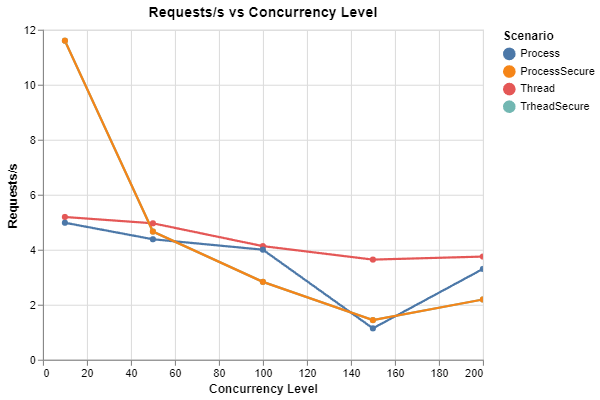
\includegraphics[width=0.6\textwidth]{res/request.png}
    \caption{Diagram Arsitektur Eksperimen}
    \label{fig:arch}
    \end{figure}

\subsubsection{Total Transactions vs. Concurrency Level}
\begin{figure}[h!]

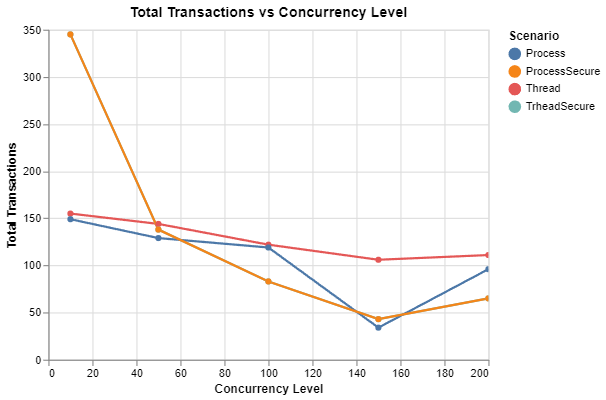
\includegraphics[width=0.6\textwidth]{res/transaction.png}
\caption{Diagram Arsitektur Eksperimen}
\label{fig:arch}
\end{figure}

Berdasarkan grafik 'Requests/s vs Concurrency Level (All Scenarios)' dan 'Total Transactions vs Concurrency Level (All Scenarios)', dapat disimpulkan:
\\\\
Thread vs. Process (Secure/Non-Secure)
\begin{itemize}
    \item \textbf{Requests/s}: Secara umum, skenario \textit{Thread} (baik \textit{secure} maupun \textit{non-secure}) memiliki \textit{Requests/s} yang lebih tinggi pada tingkat konkurensi rendah (10). Namun, seiring dengan meningkatnya konkurensi, kinerja \textit{Thread} menurun drastis, terutama untuk \textit{Thread Non-Secure}. \textit{Process Secure} dan \textit{Non-Secure} menunjukkan penurunan yang lebih gradual.
    \item \textbf{Total Transactions}: \textit{Thread} menyelesaikan lebih banyak transaksi pada konkurensi rendah, namun jumlahnya menurun tajam seiring meningkatnya konkurensi, terutama untuk \textit{Thread Non-Secure}. \textit{Process}, baik \textit{secure} maupun \textit{non-secure}, menunjukkan penurunan yang lebih lambat dan mampu menyelesaikan lebih banyak transaksi pada konkurensi yang lebih tinggi.
\end{itemize}

Secure vs. Non-Secure (Thread/Process)
\begin{itemize}
    \item \textbf{Requests/s}: Untuk \textit{Thread}, versi \textit{secure} memiliki kinerja yang sedikit lebih baik pada konkurensi rendah, namun perbedaannya tidak signifikan pada konkurensi tinggi. Untuk \textit{Process}, versi \textit{secure} secara konsisten memiliki kinerja yang sedikit lebih rendah daripada versi \textit{non-secure}.
    \item \textbf{Total Transactions}: Perbedaan antara \textit{secure} dan \textit{non-secure} tidak terlalu signifikan untuk kedua model (\textit{Thread} dan \textit{Process}) dalam hal total transaksi yang diselesaikan.
\end{itemize}


\end{document}